Enabling Lazy Shadowing for resiliency in extreme-scale computing 
brings about a number of challenges and design decisions, including the applicability of this concept to a large number of 
tasks executing in parallel, the effective way to control shadows' execution rates, and the runtime mechanisms and 
communications support to ensure efficient coordination between a 
main and its shadow.
Taking into consideration the main characteristics of compute-intensive and highly-scalable applications, we design two novel techniques, referred to as {\it shadow collocation} and {\it shadow leaping}, 
and integrate them with Shadow Replication to form a more efficient and scalable paradigm that we call Lazy Shadowing.
%in order to achieve high-tolerance to failure while minimizing delay and energy consumption.

%We consider the class of compute-intensive and strongly-scaled applications, executing on a large-scale multi-core computing infrastructure~\cite{doe_ascr_exascale_2011}. 
%We use $W$ to denote the size of an application workload, and assume that the workload is split into a set of tasks, $T$, which execute in parallel. 
%Assuming the maximum execution rate is $\sigma_{max}=1$, the failure-free completion time of the application is $W/|T|$. 
%Given the prominence of MPI in HPC environments, we assume message passing as the communication mechanism between tasks. 
%The execution is composed of a set of iterations separated by synchronization barriers. 

\section{Shadow collocation}
To control the processes' execution rate, DVFS can be applied while each process resides on one core exclusively. 
The effectiveness of DVFS, however, may be markedly 
limited by the granularity of voltage control, the number of frequencies available, and the negative effects on 
reliability~\cite{Eyerman:2011:FDU:1952998.1952999,Keller:EECS-2015-257,chandra2008defect,zhao2008reliability}. 
An alternative is to collocate multiple processes on each core while keeping all the cores executing at maximum frequency. 
Then time sharing can be used to achieve the desired execution rates for each collocated process. 
Since this approach collocates multiple processes on each  core, it simultaneously reduces the number of compute nodes required and 
reduces the power consumption. 


%We use the term core to represent the resource allocation unit (e.g., a
%CPU core, a multi-core CPU, or a cluster node), so that our algorithm is agnostic to the
%granularity of the hardware platform~\cite{casanova_inria_2012}. Each main process executes on one core exclusively to achieve maximum throughput.  
%On the other hand, we collocate multiple shadows on a single core and use time sharing to achieve the desired execution rates.
To execute an application of $M$ tasks, $N=M+S$ cores are required, where $M$ is a multiple of $S$. Each main is allocated one core (referred to as \textit{main core}), while $\alpha=M/S$ (referred to as \textit{collocation ratio}) shadows are collocated on a core (\textit{shadow core}). 
The $N$ cores are grouped into $S$ sets, each of which we call a \textit{shadowed set}. Each shadowed set contains $\alpha$ main cores and 1 shadow core.
This is illustrated in Figure~\ref{fig:sc_mapping}.  

Collocation has an important ramification with respect to the resilience of the system. Specifically, 
one failure can be tolerated in each shadowed set. If a shadow core fails, all the shadows in the 
shadowed set will be lost without interrupting the execution of the mains. 
On the other hand, if a main core fails, the associated shadow will be promoted to a new main, and all 
the other collocated shadows will be terminated to speed up the new main.
Consequently, a failure, either in main or shadow core, will result in losing all the shadows in the shadowed set, thereby losing the tolerance to any other failures. After the first failure, a shadowed set becomes \emph{vulnerable}\footnote{Rejuvenation techniques, such as restarting the lost shadows from the state of current mains on spare cores, can be used to eliminate vulnerability.}. 
 
\begin{figure}[!b]
  \begin{center}
    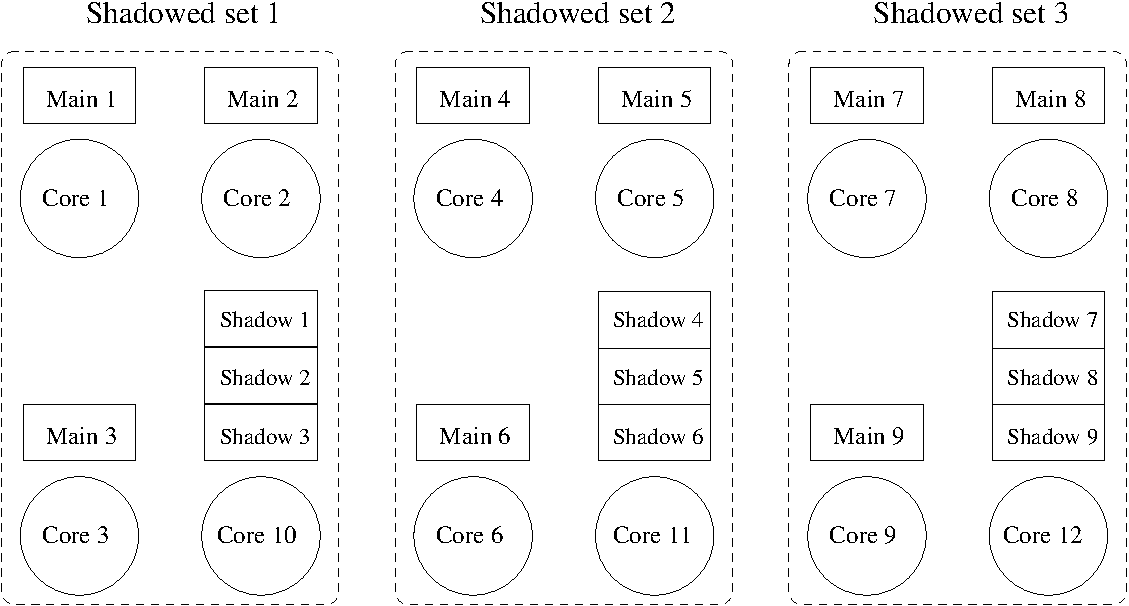
\includegraphics[width=0.6\columnwidth]{Figures/sc_mapping.pdf}
  \end{center}
  %\vskip -0.25in 
  \caption{An example of collocation. $N=12$, $M=9$, $S=3$.}
  \label{fig:sc_mapping}
\end{figure}


\section{Shadow leaping}
\label{sec:leaping_shadows}

As the shadows execute at a lower rate, failures will incur delay for recovery. This problem deteriorates as dependencies incurred by messages and synchronization barriers would propagate the delay of one task to others.  
Fortunately, keeping the mains running at normal rate provides an opportunity for the shadows to benefit from the faster execution of their mains. By copying the state of each main to its shadow, which is similar to the process of storing a checkpoint in a buddy in \cite{zheng_2004_ftccharm}, forward progress is achieved for the shadows with minimized time and energy. This technique, referred to as \textit{shadow leaping}, effectively limits the distance between main and shadow in progress. 
As a result, the recovery time after a failure, which depends on the distance between the failing main 
and its shadow, is also reduced. 
More importantly, 
we opportunistically overlap shadow leaping with failure recovery to avoid extra overhead. 

Assuming a failure occurrence at time $t_f$, Figure~\ref{fig:leap} shows the concept of shadow leaping. 
Upon failure of a main process, its associated shadow speeds up to minimize the impact of failure recovery on the other tasks' progress, as illustrated in Figure~\ref{fig:jump1}. 
At the same time, as shown in Figure~\ref{fig:jump2}, the remaining main processes continue execution until the barrier at $W_{syn}$, and then become idle until $t_r$. 
Shadow leaping opportunistically takes advantage of this idle time to {\it leap forward} the shadows, so that  
all processes, including shadows, can resume execution from a consistent point afterwards. 
Shadow leaping increases the shadow's rate of progress, at a minimal energy cost. Consequently, it reduces significantly the likelihood of a shadow falling excessively behind, thereby ensuring fast recovery while minimizing the total energy consumption.

\begin{figure}[!t]
	\begin{center}
        \subfigure[Faulty task behavior.]
		{
			\label{fig:jump1}
			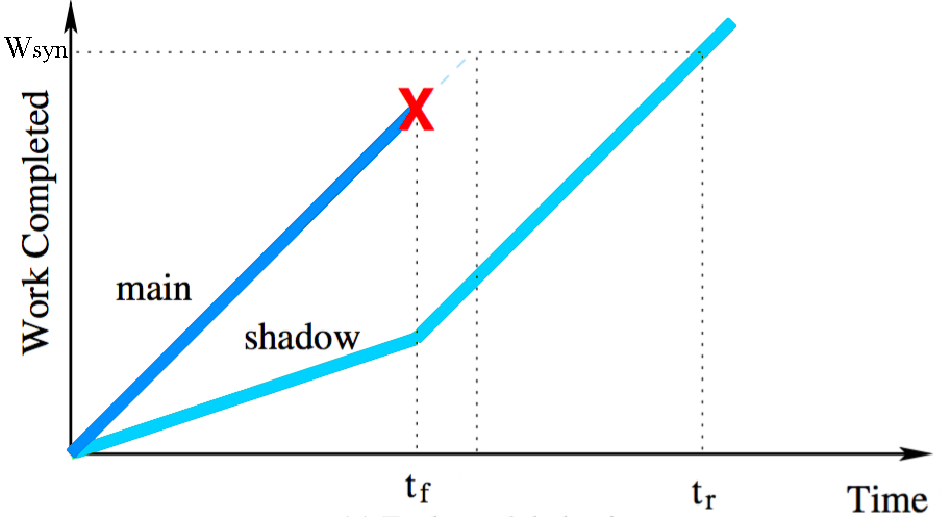
\includegraphics[width=0.4\columnwidth]{Figures/jump1.pdf}
		}
		\subfigure[Non-faulty task behavior.]
		{
			\label{fig:jump2}
			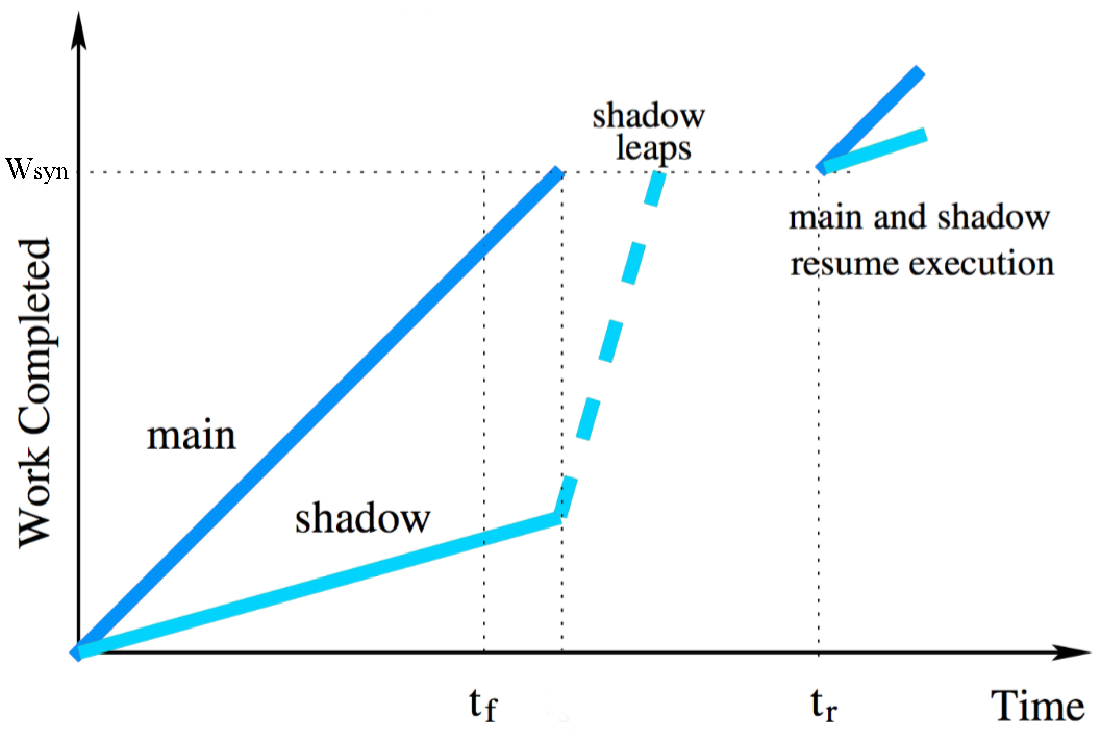
\includegraphics[width=0.4\columnwidth]{Figures/jump2.pdf}
		}
	\end{center}
	\caption{The illustration of shadow leaping.}
	\label{fig:leap}
\end{figure}
\vskip -0.5in
%\section{Analytical framework}
%
%In the following we develop analytical models to quantify the expected performance of Lazy Shadowing, as well as prove the bound on performance loss due to failures. 
%All the analysis below is under the assumption that there are a total of $N$ cores, and $W$ is the application workload.  
%$M$ of the $N$ cores are allocated for main processes, each having a workload of $w=\frac{W}{M}$, and the rest $S$ cores are for the collocated shadow processes. %For process replication,
%Note that process replication is a special case of Lazy Shadowing where $\alpha=1$, so 
%$M=S=\frac{N}{2}$ and $w=\frac{2W}{N}$. 
%
%An application has to roll back when all replicas of a task have been lost. We call this an application fatal failure, which is inevitable even when every process is replicated. 
%In order to take into account the overhead of rollback in the calculation of completion time and energy consumption, we first 
%study the probability of application fatal failure. 
%We use 
%$f(t)$ to denote the failure probability density function of each core, and then $F(t) = \int_0^tf(\tau)d\tau$ is the probability that a core fails in the next $t$ time. 
%Since each shadowed set can tolerate one failure, 
%then the probability that a shadowed set with $\alpha$ main cores and 1 shadow core does not fail by time $t$ is the probability of no failure plus the probability of one failure, i.e., 
%
%\begin{equation}
%	P_g = \Big(1-F(t)\Big)^{\alpha+1} + {{\alpha+1} \choose 1}F(t)\times \Big(1-F(t)\Big)^{\alpha}
%\end{equation}
%and the probability that an fatal failure occurs to an application using $N$ cores within $t$ time is the complement of the probability that
%none of the shadowed sets fails, i.e.,
%
%\begin{equation}
%	P_a = 1 - ({P_g})^{S}
%\end{equation}
%where $S=\frac{N}{\alpha+1}$ is the number of shadowed sets.
%The application fatal failure probability can then be calculated by using $t$ equal to the expected completion time of the application, which will be modeled in the next subsection.
%
%There are two types of delay due to failures. If a failure does not lead to an application fatal failure, the delay corresponds to the catching up of the shadow of the failing main (see Figure~\ref{fig:jump1}). Otherwise, a possible larger (rollback) delay will be introduced by an application fatal failure. In the following we consider both delays step by step. 
%First we discuss the case of $k$ failures without application fatal failure. Should a failure occur during the recovery of a previous failure, its recovery would overlap with the ongoing recovery. To study the worst case behavior, we assume failures do not overlap, so that the execution is split into $k+1$ intervals, as illustrated in Figure~\ref{fig:progress}. 
%$\Delta_i$ ($1\le i \le k+1$) represents the $i^{th}$ execution interval, and $\tau_i$ ($1\le i \le k$) is the recovery time after $\Delta_i$. 
%
%\begin{figure}[!t]
%	\begin{center}
%		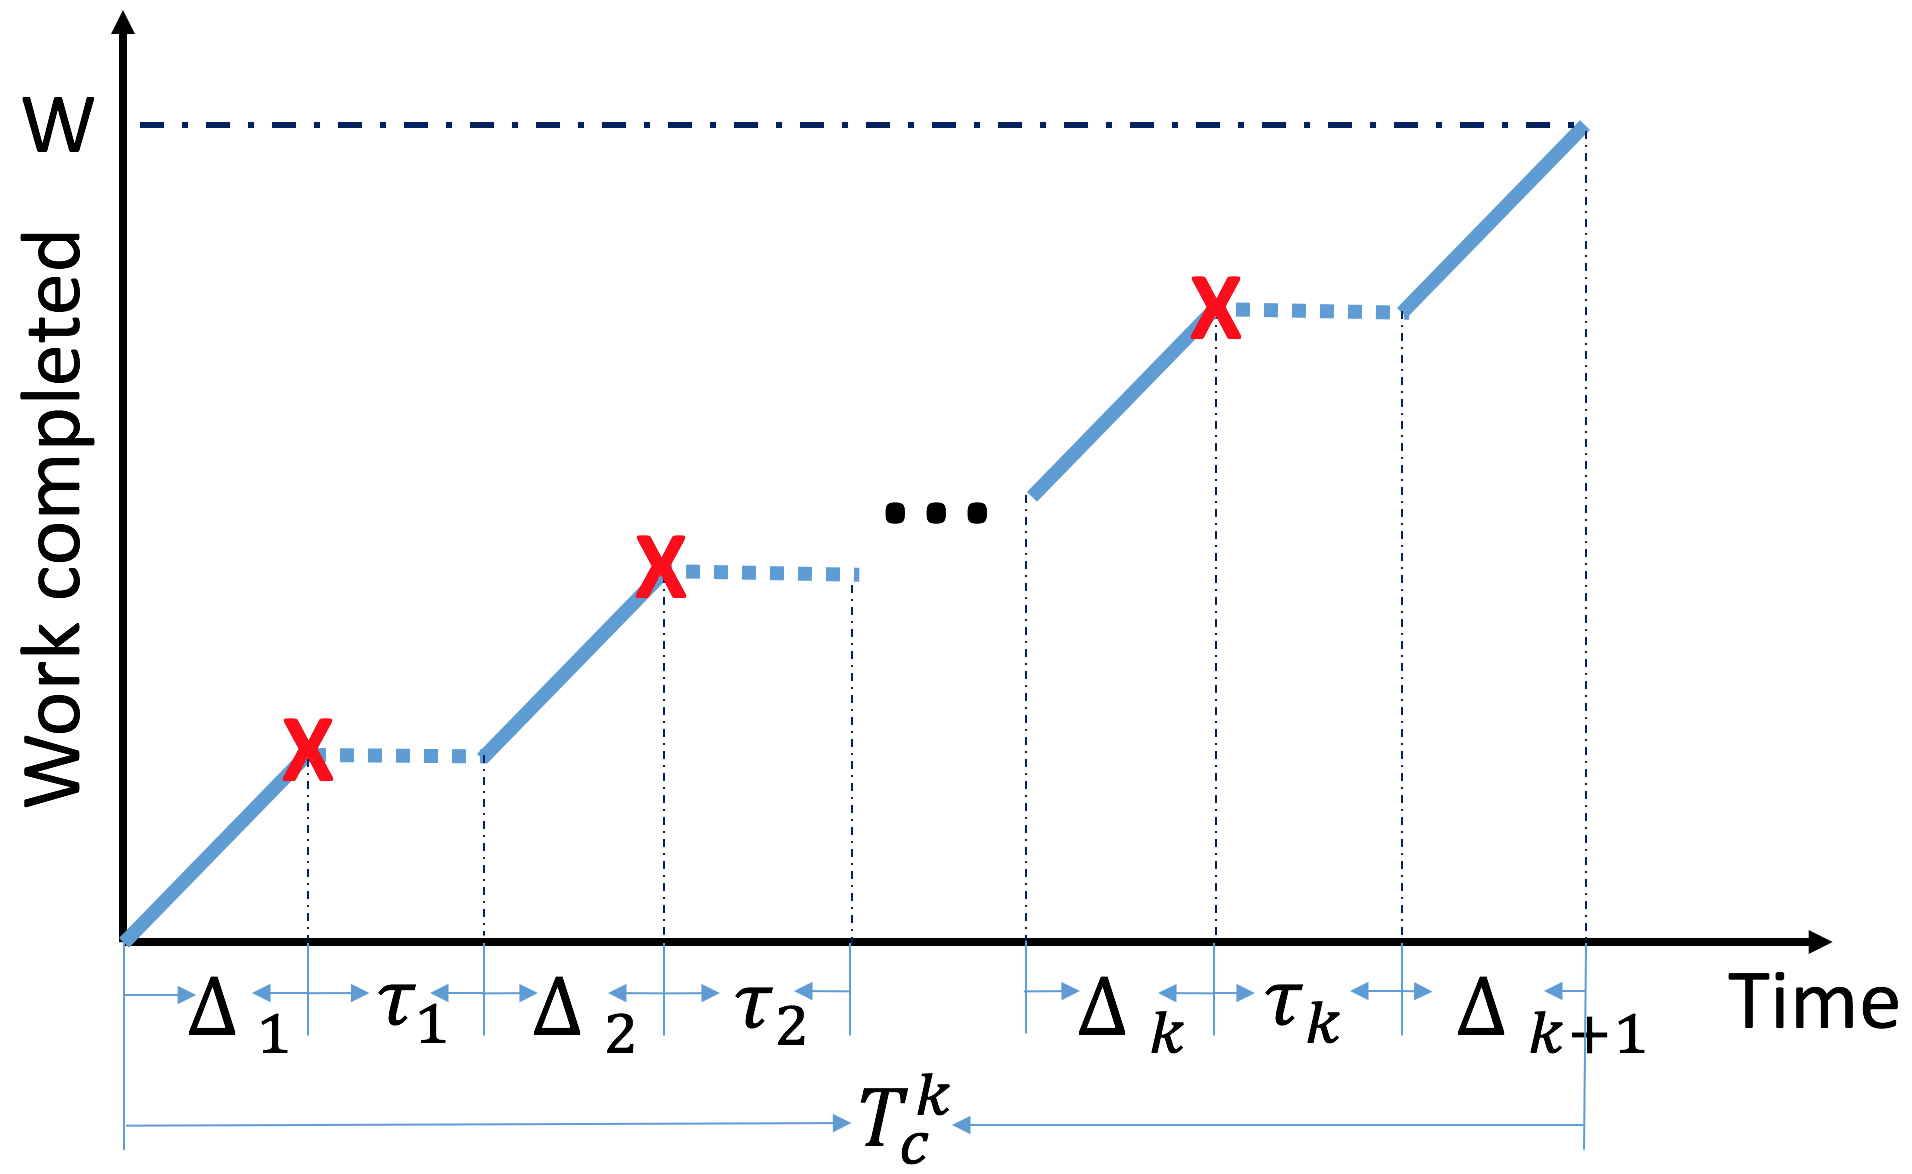
\includegraphics[width=0.7\columnwidth]{Figures/progress}
%	\end{center}
%	%\vskip -0.22in 
%	\caption{Application's progress with shadow catching up delays.}
%	\label{fig:progress}
%\end{figure}
%
%
%The following theorem expresses the completion time, $T_c^k$, as a function of $k$.
%
%\begin{theorem}
%Assuming that failures do not overlap and no application fatal failure occurs, then using Lazy Shadowing, 
%	$$T_c^k = w + (1-\sigma_s^b)\sum_{i=1}^k\Delta_i$$
%\end{theorem}
%\begin{proof}
%
%Lazy Shadowing guarantees that all the shadows reach the same execution point as the mains (See Figure~\ref{fig:leap}) after a previous recovery, so every recovery time is proportional to its previous execution interval. %, which is $\Delta_i$. 
%That is, $\tau_i = \Delta_i \times (1 - \sigma_s^b)$. 
%According to Figure~\ref{fig:progress}, the completion time with $k$ failures is 
%	$T_c^k = \sum_{i=1}^{k+1}\Delta_i + \sum_{i=1}^k\tau_i = w + (1-\sigma_s^b)\sum_{i=1}^k\Delta_i$
%\end{proof}
%
%Although it may seem that the delay would keep growing with the number of failures, 
%it turns out to be well bounded, as a benefit of shadow leaping: 
%
%\begin{corollary}
%The delay induced by failures is bounded by $(1-\sigma_s^b)w$.
%\end{corollary}
%\begin{proof}
%From above theorem we can see the delay from $k$ failures is $(1-\sigma_s^b)\sum_{i=1}^k\Delta_i$. It is straightforward that, for any non-negative integer of $k$, we have the equation $\sum_{i=1}^{k+1}\Delta_i= w$. As a result, 
%$\sum_{i=1}^{k}\Delta_i = w - \Delta_{k+1} \le w$. Therefore, $(1-\sigma_s^b)\sum_{i=1}^k\Delta_i \le (1-\sigma_s^b)w$.
%\end{proof}
%
%Typically, the number of failures to be encountered is stochastic. Given a failure distribution, however, we can calculate the probability for a specific value of $k$. We assume that failures do not occur during recovery, so the failure probability of a core during the execution can be calculated as $P_c = F(w)$. Then the probability that there are $k$ failures among the $N$ cores is 
%\begin{equation}
%\begin{split}
%P_s^{k}= & \dbinom{N}{k}{P_c}^k(1-P_c)^{N-k} \\
%\end{split}
%\end{equation}
%
%The following theorem expresses the expected completion time, $T_{total}$, considering all possible number of failures. 
%
%\begin{theorem}
%Assuming that failures do not overlap, then using Lazy Shadowing,
%$T_{total} = T_{c} / (1 - P_a)$, where $T_{c} = \sum_{i} T_{c}^{i} \cdot P_s^{i}$.
%\end{theorem}
%\begin{proof}
%Without application fatal failure, the completion time considering all possible values of $k$ can be averaged as $T_{c} = \sum_{i} T_{c}^{i} \cdot P_s^{i}$. If an application fatal failure occurs, however, the application needs to roll back to the beginning. With the probability of rollback calculated as $P_a$ in Section~\ref{anal_app_fail}, the total expected completion time is $T_{total} = T_{c} / (1 - P_a)$.
%\end{proof}
%
%Process replication is a special case of Lazy Shadowing where $\alpha=1$, so we can use the above theorem to derive the expected completion time for process replication using the same amount of cores:
%
%\begin{corollary}
%The expected completion time for process replication is $T_{total} = 2W/N / (1 - P_a)$.
%\end{corollary}
%\begin{proof}
%Using process replication, half of the available cores are dedicated to shadows so that the workload assigned to each task is significantly increased, i.e., $w=2W/N$. Different from cases where $\alpha \ge 2$, failures do not incur any delay except for application fatal failures. %, since the replicas are executing at the same rate as the main processes. 
%As a result, without application fatal failure the completion time under process replication is constant regardless of the number of failures, i.e., $T_c=T_c^k=w=2W/N$. Finally, the expected completion time considering the possibility of rollback is $T_{total} = T_c / (1 - P_a) = 2W/N / (1 - P_a)$.
%\end{proof}
%
%Power consumption consists of two parts, dynamic power, $p_d$, which exists only when a core is executing, and static power, $p_s$, which is constant as long as the machine is on. This can be modeled as $p = p_d + p_s$. Note that in addition to CPU leakage, other components, such as memory and disk, also contribute to static power. 
%
%
%For process replication, all cores are running all the time until the application is complete. Therefore, the expected energy consumption, $En$, is proportional to the expected execution time $T_{total}$: 
%\begin{equation}
%%En = N * p * T_{total}
%En = N \times p \times T_{total}
%\label{eq:exp_energy1}
%\end{equation} 
%
%Even using the same amount of cores, Lazy Shadowing can save power and energy, since main cores are idle during the recovery time after each failure, and the shadows can achieve forward progress through shadow leaping. During normal execution, all the cores consume static power as well as dynamic power. During recovery time, however, the main cores are idle and consume only static power, while the shadow cores first perform shadow leaping and then become idle. Altogether, the expected energy consumption for Lazy Shadowing can be modeled as 
%\begin{equation}
%En = N \times p_s \times T_{total} + N \times p_d \times w + S \times p_{l} \times T_l.
%%En = N * p_s * T_{total} + N * p_d * w + S * p_{l} * T_l.
%\label{eq:exp_energy2}
%\end{equation}
%with $p_{l}$ denoting the dynamic power consumption of each core during shadow leaping and $T_l$ the expected total time spent on leaping.

\section{Performance evaluation}
We develop analytical models to quantify
the expected performance of Lazy Shadowing, as well as
prove the bound on performance loss due to failures.
 Please refer to~\cite{cui_2016_scalcom} for details. 
Careful analysis of the models leads us to identify several important factors that determine the performance. These factors can be classified into three categories, i.e., system, application, and algorithm. The system category includes static power ratio $\rho$ ($\rho=p_s/p$), total number of cores $N$, and MTBF of each core; the application category is mainly the total workload, $W$; and shadowing ratio $\alpha$ in the algorithm category determines the number of main cores and shadow cores ($N=M+S$ and $\alpha=M/S$). In this section, we evaluate each performance metric of Lazy Shadowing, 
 %using the models above, 
 with the influence of each of the factors considered.

We compare with both process replication and checkpointing. %, assuming the same number of cores to use. 
The completion time with checkpointing is calculated with Daly's model~\cite{daly_fgcs_2006} assuming 10 minutes for both checkpointing time and restart time. %The energy consumption is then derived with Equation~\ref{eq:exp_energy1}. 
It is important to point out that we always assume the same number of cores available to use, so that process replication and Lazy Shadowing do not use extra cores for the replicas. 

%It is clear from THEOREM 1 that the total recovery delay $\sum_{i=1}^k\tau_i$ is determined by the execution time $\sum_{i=1}^k\Delta_i$, independent of the distribution of failures. 
%% which determines the individual value of $\Delta_i$. 
%Therefore, our models are generic with no assumption about failure probability distribution, and the expectation of the total delay from all failures is the same as if failures are uniformly distributed~\cite{daly_fgcs_2006}. Specifically, $\Delta_i = w/(k+1)$, and $T_c^k = w + w*(1-\sigma_s^b)*\frac{k}{k+1}$. Further, we assume that each shadow gets a fair share of its core's execution rate so that $\sigma_s^b = \frac{1}{\alpha}$.
%To calculate Equation~\ref{eq:exp_energy2}, we assume that the dynamic power during shadow leaping is twice of that during normal execution, i.e., $p_{l}=2*p_d$, and the time for shadow leaping is half of the recovery time, i.e., $T_l=0.5*(T_{total} - w)$ 

The first study uses $N=1$ million cores, %effectively simulating the future extreme-scale computing environment, and assumes that $W=1$ million hours. 
$W=1$ million hours, and static power ratio $\rho=0.5$.
Our results show that at extreme-scale, the completion time and energy consumption of checkpointing are orders of magnitude larger than those of Lazy Shadowing and process replication. Thus, we choose not to plot a separate graph for checkpointing in the interest of space. 
Figure~\ref{fig:t32} reveals that the most time efficient choice largely depends on MTBF. 
%More specifically, process replication consumes less time when MTBF is low while otherwise Lazy Shadowing is more efficient.
When MTBF is high, Lazy Shadowing requires less time as more cores are used for main processes and less workload is assigned to each process. As MTBF decreases, process replication outperforms Lazy Shadowing as a result of the increased likelihood of rollback for Lazy Shadowing.
In terms of energy consumption, Lazy Shadowing has a much larger advantage over process replication. %For MTBF from 2 to 25 years, Lazy Shadowing with $\alpha=5$ can achieve 9.6-17.1\% energy saving, while the saving increases to 13.1- 23.3\% for $\alpha=10$. The only exception is when MTBF is extremely low (1 year), Lazy Shadowing with $\alpha=10$ consumes more energy because of extended execution time.

\begin{figure}[!t]
	%\captionsetup{justification=centering}
	\begin{center} 
		\subfigure[Expected completion time]
		{
			\label{fig:t32}
			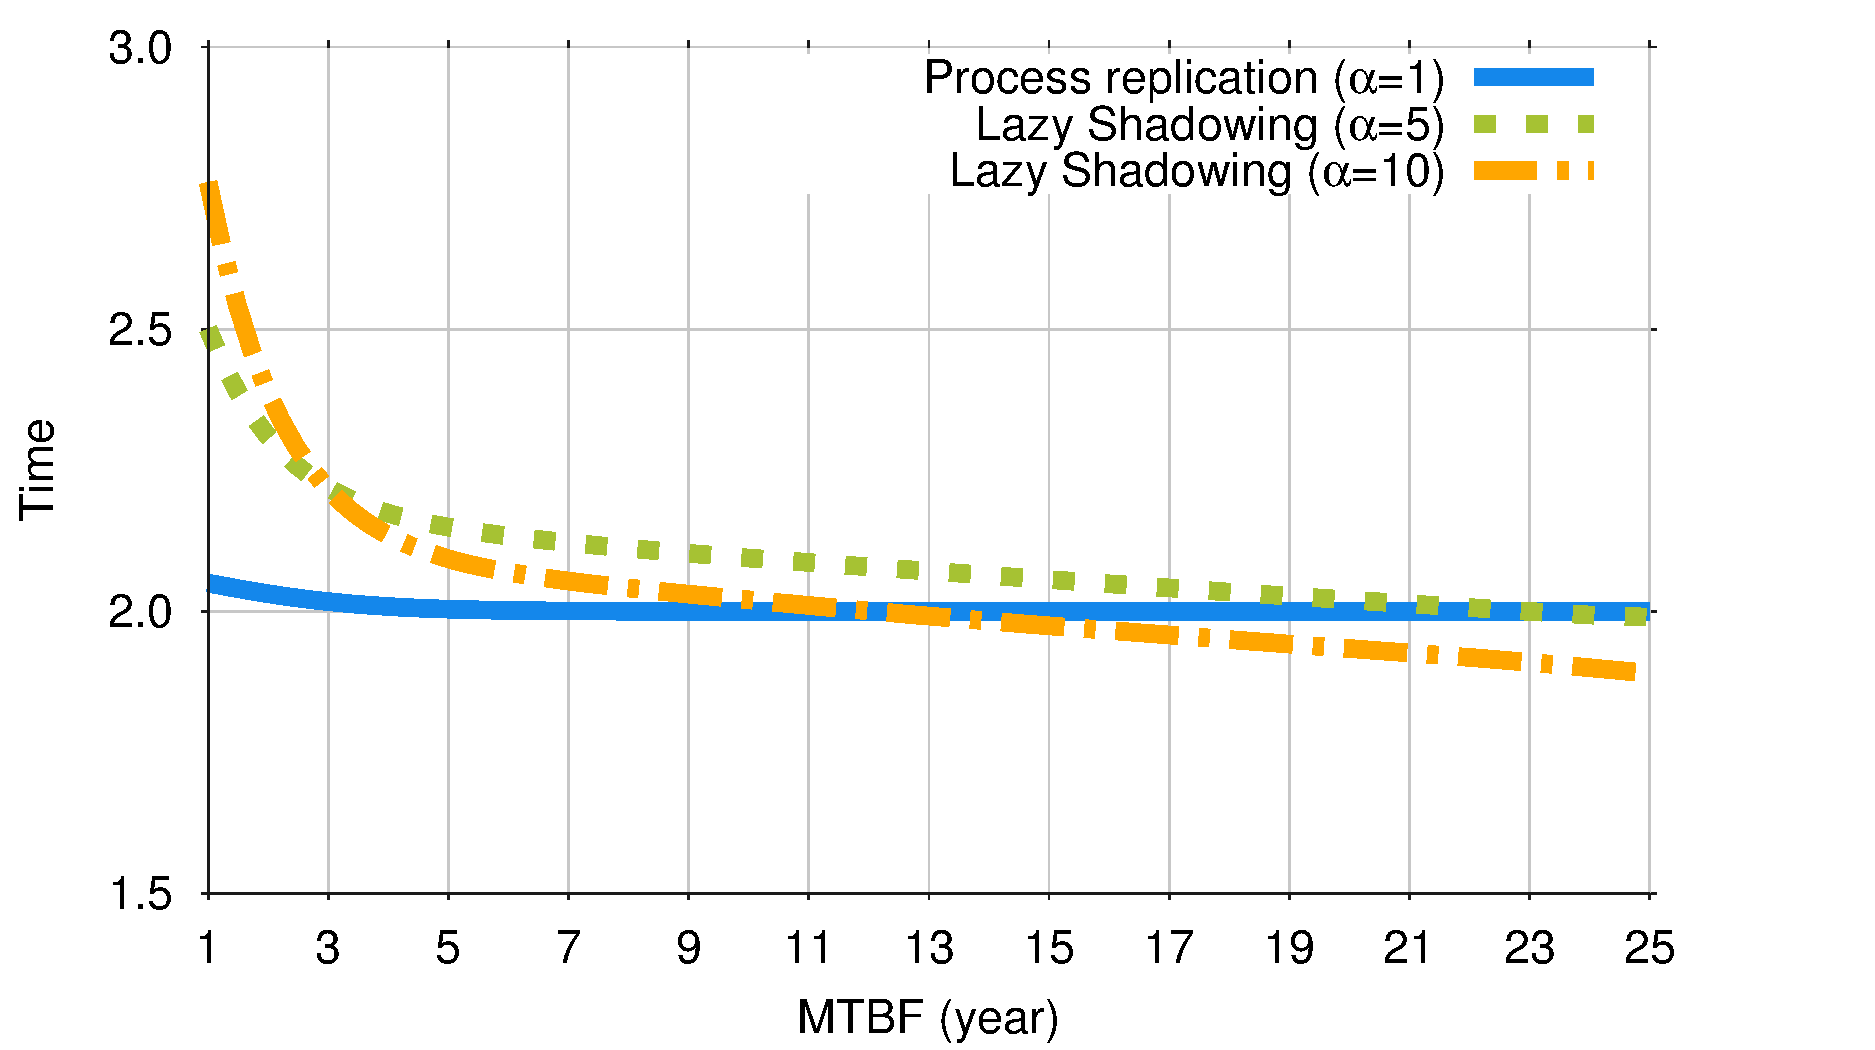
\includegraphics[width=0.4\columnwidth]{Figures/gen_time.pdf}
			%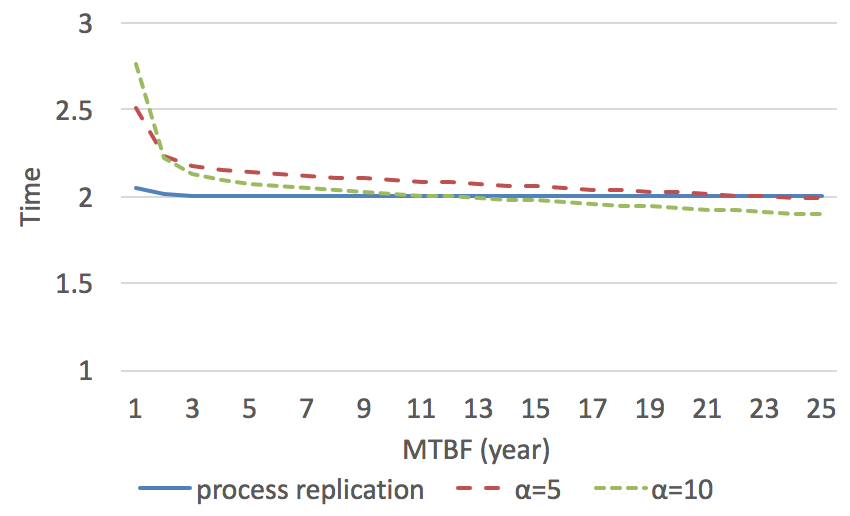
\includegraphics[width=0.7\columnwidth]{Figures/tt32}
		} 
		\subfigure[Expected energy consumption]
		{
			\label{fig:e32}
			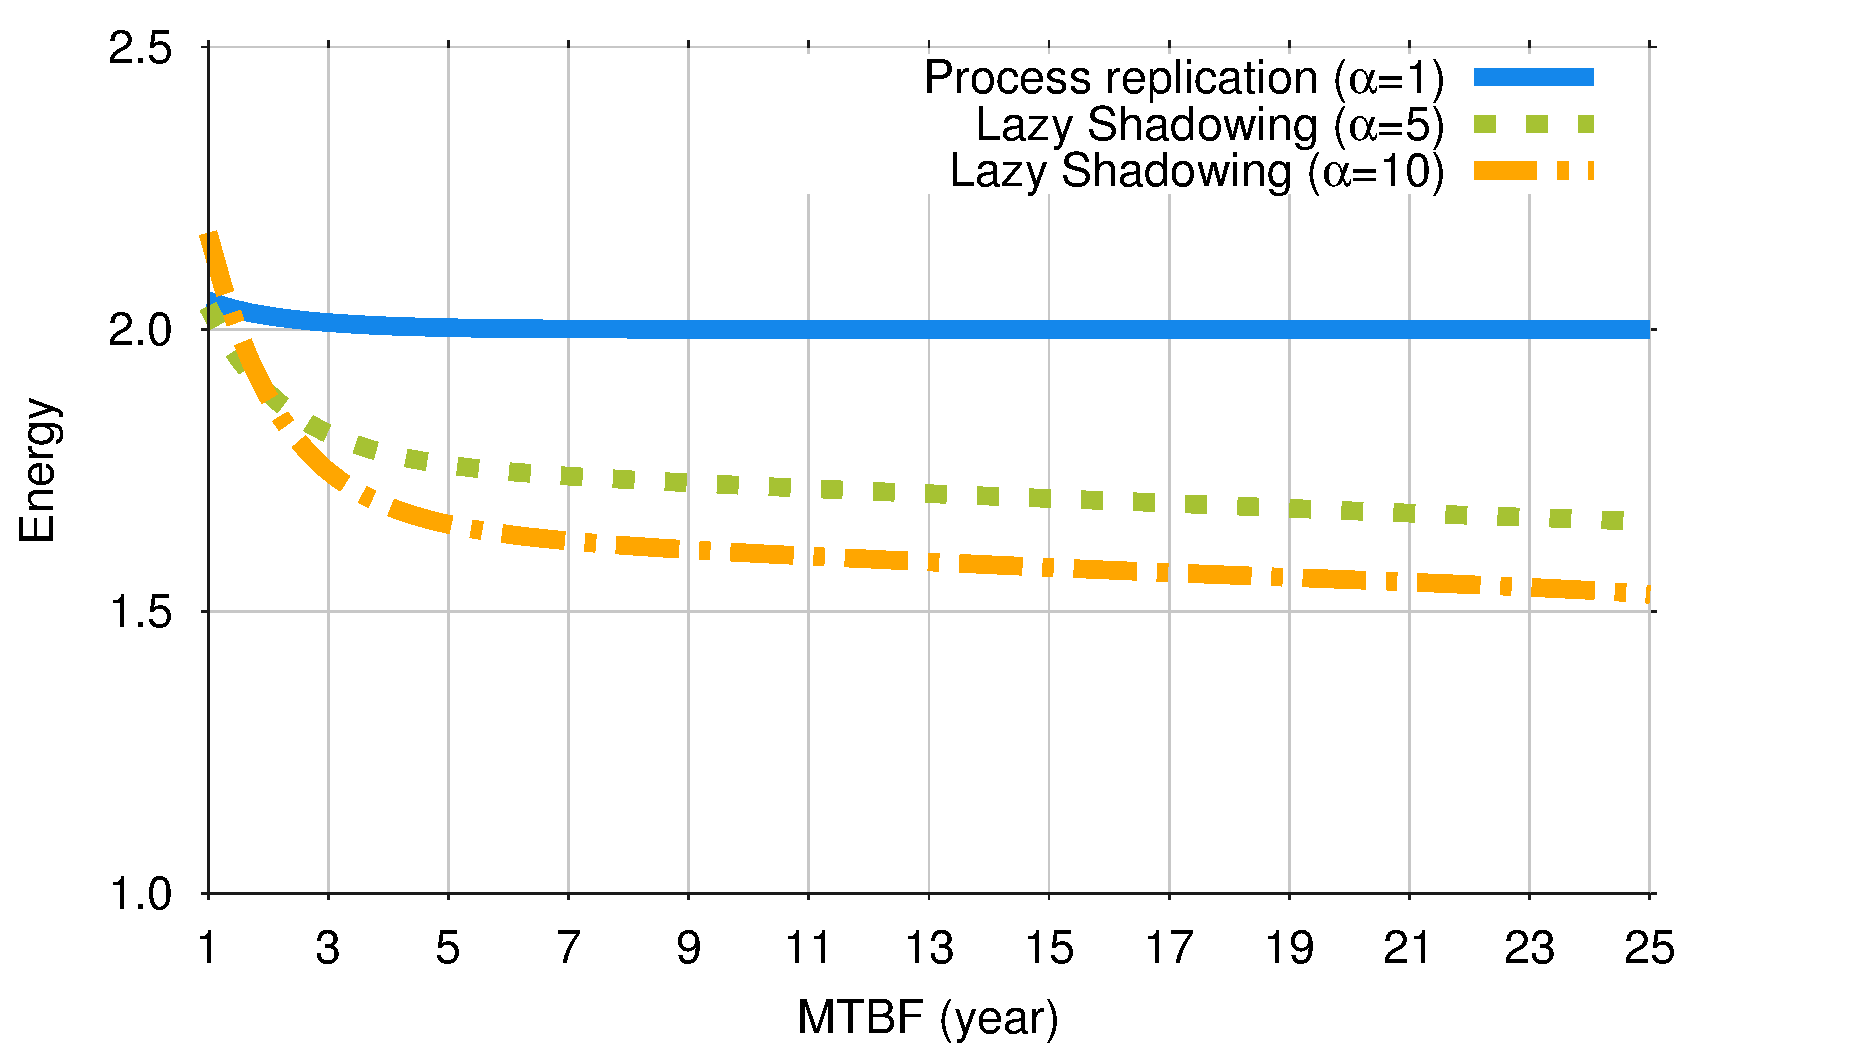
\includegraphics[width=0.4\columnwidth]{Figures/gen_energy.pdf}
			%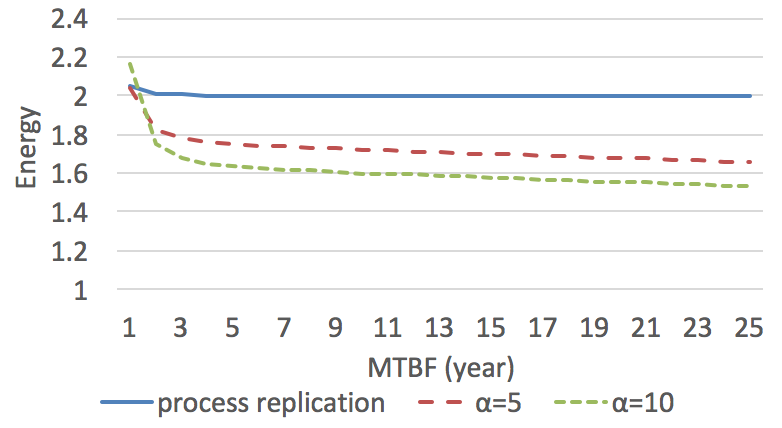
\includegraphics[width=0.7\columnwidth]{Figures/te32}
		} 
		\caption{Comparison of time and energy for different core level MTBF. $W=10^6$ hours, $N=10^6$, $\rho=0.5$.}
	\end{center}
	%\vskip -0.22in 
	\label{fig:com3}
\end{figure}

The system scale, measured in number of cores, has a direct impact on the failure rate seen by the application. To study its impact, we vary $N$ from 10,000 to 1,000,000 with $W$ scaled proportionally, i.e., $W=N$. When MTBF is 5 years, the results are shown in Figure~\ref{fig:n5}. Please note that the time and energy for checkpointing when $N=1,000,000$ are beyond the scope of the figures, so we mark their values on top of their columns. When completion time is considered, Figure~\ref{fig:nt5} clearly shows that each of the three fault tolerance alternatives has its own advantage. %Specifically, checkpointing is the best choice for small systems at the scale of 10,000 cores, Lazy Shadowing outperforms others for systems with 100,000 cores, while process replication has slight advantage over Lazy Shadowing for larger systems. 
On the other hand, Lazy Shadowing wins for all system sizes when energy consumption is the objective. 

%When MTBF is changed to 25 years, the performance of checkpointing improves a lot, but is still much worse than that of the other two approaches. Lazy Shadowing benefits much more than process replication from the increased MTBF. As a result, Lazy Shadowing is able to achieve shorter completion time than process replication when $N$ reaches 1,000,000.

\begin{figure}[!t]
	%\captionsetup{justification=centering}
	\begin{center}
		\subfigure[Expected completion time]
		{
			\label{fig:nt5}
			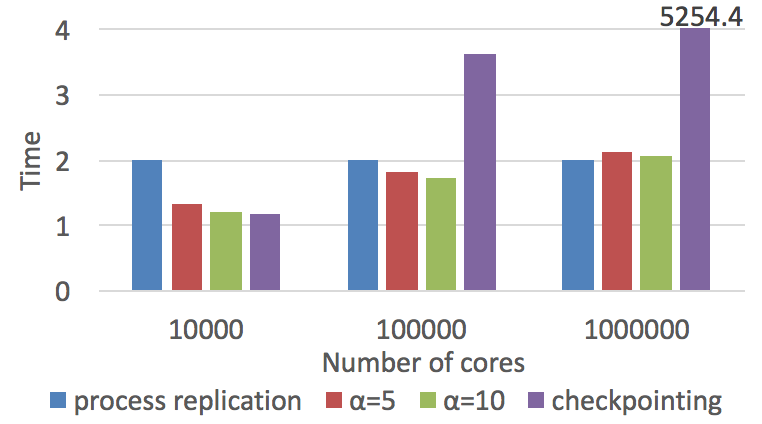
\includegraphics[width=0.4\columnwidth]{Figures/tnt5}
		} 
		\subfigure[Expected energy consumption]
		{
			\label{fig:ne5}
			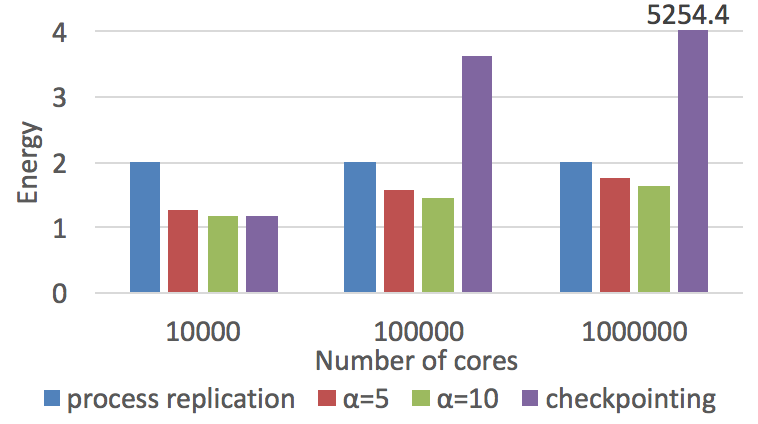
\includegraphics[width=0.4\columnwidth]{Figures/tne5}
		} 
	\end{center}
	%\vskip -0.22in 
	\caption{Comparison of time and energy for different number of cores. $W=N$, MTBF=5 years, $\rho=0.5$.}
	\label{fig:n5}
\end{figure}

With various architectures and organizations, servers
vary in terms of
power consumption. The static power ratio $\rho$ is used to abstract the
amount of static power consumed versus dynamic power. 
%$\rho$ does not impact the completion time, but power and energy consumption.
Considering modern systems, we vary $\rho$ from 0.3 to 0.7 and study its effect
on the expected energy consumption. The results for Lazy Shadowing with $\alpha=5$ are normalized to that of process replication and shown in 
Figure~\ref{fig:power_ratio}. 
%The results for other values of $\alpha$ have similar behavior and thus are not shown. 
Lazy Shadowing achieves
more energy saving when the static power ratio is low, since it saves dynamic 
power but not static power. %When static power ratio is low ($\rho=0.3$), Lazy Shadowing
%is able to save 20\%-24\% energy for the MTBF of 5 to 25 years. The saving decreases to 5\%-11\% when $\rho$ reaches 0.7. 

\begin{figure}[!t]
	%\captionsetup{justification=centering}
	\begin{center}
		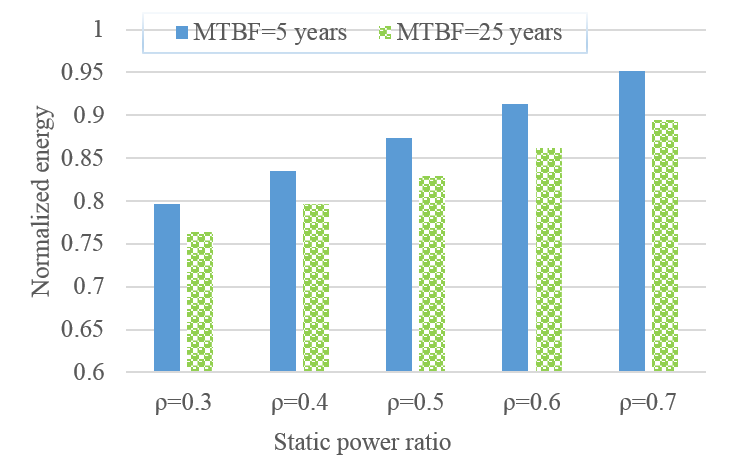
\includegraphics[width=0.7\columnwidth]{Figures/ts_power_5}
	\end{center}
	%\vskip -0.22in 
	\caption{Impact of static power ratio on energy consumption. $W=10^6$ hours, $N=10^6$, $\alpha$=5.}
	\label{fig:power_ratio}
\end{figure}

\section{Summary}

%As the scale and complexity of HPC systems continue to increase, both the failure rate and power consumption are expected to increase dramatically, making it extremely challenging to deliver extreme-scale computing performance efficiently. Existing fault tolerance methods rely on either time or hardware redundancy. Neither of them appeals to the next generation of supercomputing, as the first approach may incur significant delay while the second one constantly wastes over 50\% of the system resources.

In this work, we present a comprehensive discussion of the techniques that enable Lazy Shadowing to achieve scalable resilience in future extreme-scale computing systems. In addition, we develop a series of analytical models to assess its performance in terms of reliability, completion time, and energy consumption. 
Through comparison with existing fault tolerance approaches, we identify the scenarios where each of the alternatives should be chosen for best performance.










